%%=====================================================================
%%  RT-IIPF : Real-Time Inline Payment Fraud Mitigation Framework
%%  IEEEtran conference format -- self-contained, compiles with pdflatex
%%  Build:  pdflatex main && bibtex main && pdflatex main && pdflatex main
%%=====================================================================
\documentclass[conference]{IEEEtran}
\IEEEoverridecommandlockouts

\usepackage{cite}
\usepackage{amsmath,amssymb,amsfonts}
\usepackage{algorithmic}
\usepackage{graphicx}
\usepackage{textcomp}
\usepackage{xcolor}
\usepackage{booktabs}
\usepackage{array}
\usepackage{tikz}
\usetikzlibrary{positioning,arrows.meta,fit,backgrounds}
\usepackage{url}

% Currency macro: portable across distributions (no rupee-glyph package
% dependency, and unambiguous for an international readership).
\newcommand{\INR}[1]{\mbox{INR~#1}}

\def\BibTeX{{\rm B\kern-.05em{\sc i\kern-.025em b}\kern-.08em
    T\kern-.1667em\lower.7ex\hbox{E}\kern-.125emX}}

\begin{document}

\title{RT-IIPF: A Real-Time Inline Payment Fraud Mitigation
Framework Using Fused Isolation Forests and Local Outlier Factors}

\author{
\IEEEauthorblockN{[Author One]}
\IEEEauthorblockA{\textit{School of Computing} \\
\textit{Sathyabama Institute of Science and Technology}\\
Chennai, India \\
[email@domain]}
\and
\IEEEauthorblockN{[Author Two]}
\IEEEauthorblockA{\textit{School of Computing} \\
\textit{Sathyabama Institute of Science and Technology}\\
Chennai, India \\
[email@domain]}
}

\maketitle

\begin{abstract}
Instant payment networks settle irrevocably, so a control that scores a
transaction after commit acts on funds that have already moved. This
paper presents RT-IIPF, which evaluates a payment inside the database
transaction while both ledger rows are held under
\texttt{PESSIMISTIC\_WRITE} locks and the debit remains uncommitted; a
fraudulent transfer is rolled back atomically and never persists in the
ledger. Scoring fuses three tiers: rules whose thresholds are derived
from training-distribution quantiles, an Isolation Forest ($M=200$,
$\psi=256$), and a Local Outlier Factor estimator ($k=20$) over a fixed
$40{,}000$-point reference set in $67$ dimensions. The fused score is
$\max(0.2\,S_{\mathrm{IF}} + 0.8\,S_{\mathrm{LOF}},\,R)$, thresholded at
$\tau = 0.802$ fixed by a matched false-positive-rate sweep at
$\mathrm{FPR}=0.0086$. On $50{,}000$ clean and $400$ injected
transactions the deployed configuration attains recall $0.745$,
precision $0.380$, and F1 $0.503$; a density-only configuration reaches
precision $0.409$, and we report both. Account lockout commits through
an independent \texttt{REQUIRES\_NEW} transaction and survives the
ledger rollback. Inference costs $17.3$\,ms and end-to-end switch
latency is $22.4$\,ms at unit concurrency, with single-worker p95
within a $500$\,ms budget up to $25$ concurrent clients. Contended and
uncontended throughput are statistically indistinguishable, so the
system is not lock-bound.
\end{abstract}

\begin{IEEEkeywords}
Payment systems, anomaly detection, isolation forest, local outlier
factor, real-time switches, transactional rollback.
\end{IEEEkeywords}

%%=====================================================================
\section{Introduction}
\label{sec:introduction}

Instant retail payment networks settle irrevocably. Once a Unified
Payments Interface (UPI) transfer commits, the funds are available to
the beneficiary within seconds and recovery depends on intermediary
cooperation rather than on reversal. The interval during which a
payment can be stopped at zero cost is the interval before the database
transaction commits, and that interval is measured in milliseconds.

Most deployed fraud controls do not operate inside it. They score a
transaction after settlement and raise a case, which converts a
detection problem into a recovery problem. This work places the scoring
decision before the commit boundary and treats the resulting latency as
the design constraint to be measured.

\subsection{Operational Constraints}
\label{subsec:intro_constraints}

A payment switch allocates a fixed processing window to each
authorisation. Any inline control consumes part of that window, and
because the control executes while ledger rows are held under write
locks, it also extends the period during which those accounts are
unavailable to concurrent transactions. The cost of an inline detector
is therefore twofold: response latency and lock occupancy.

We adopt a round-trip budget of $500$\,ms as the design target for the
complete authorisation path, and report measured latency against it
throughout Section~\ref{sec:evaluation}.\footnote{The $500$\,ms figure
is this work's engineering budget. A citation to the governing network
specification should replace this note before submission.} Two
consequences follow. A detector whose inference cost approaches the
budget cannot be deployed inline regardless of its accuracy. A detector
whose cost is modest but whose variance is high will breach the budget
on its tail, which is the operationally relevant case.

\subsection{Research Gap}
\label{subsec:intro_gap}

Two established approaches sit on either side of the requirement.

Batch and near-real-time pipelines evaluate transactions after
settlement. They impose no latency on the authorisation path and can
apply arbitrarily expensive models, but they act on funds that have
already moved. Their output is a chargeback or recovery workflow whose
success is not controlled by the detector.

Deep sequential architectures---recurrent networks over transaction
histories~\cite{jurgovsky2018}, and graph networks over counterparty
structure~\cite{dou2020}---model behavioural context that
per-transaction features cannot express. Their inference cost and their
dependence on assembling a history or neighbourhood at scoring time
place them outside a millisecond-scale window held under a write lock.
They are additionally supervised, and therefore require labels that are
scarce for novel attack patterns and that arrive only after the fraud
has been reported.

The gap is a detector that is cheap enough to execute inside the lock
window, does not require labels, and produces a decision the
transaction manager can act on before commit.

\subsection{Contributions}
\label{subsec:contributions}

This paper makes three contributions, each validated against a running
implementation rather than a simulation.

\textbf{C1: An inline hybrid inference pipeline.} We combine a
deterministic rule tier with an unsupervised pair of detectors---an
Isolation Forest and a Local Outlier Factor estimator with $k=20$
calibrated against a fixed reference set of $|\mathcal{R}|=40{,}000$
points in $d=67$ dimensions. The tiers are fused by a weighted blend
floored by the rule risk and thresholded at $\tau = 0.802$, fixed by a
matched false-positive-rate sweep. The pipeline is stateless and
deterministic, which is required for the verdict to be reproducible
during audit.

\textbf{C2: A decoupled switch architecture preserving a security
invariant under rollback.} A Java~21 / Spring~Boot coordinator owns the
ledger, the locks, and the commit decision; a containerised FastAPI node
owns inference and holds no ledger state. When the pipeline returns a
fraud verdict, the account lock and the audit record are committed
through an independent \texttt{REQUIRES\_NEW} transaction that completes
before the financial transaction is rolled back. The resulting
invariant---security state persists while the ledger is left
arithmetically unchanged---is stated formally in
Section~\ref{subsec:requiresnew} and verified experimentally.

\textbf{C3: Measurement of the inline cost, including negative
results.} We report per-tier ablation at matched false-positive rate, a
controlled sweep establishing that the learned score is not monotone in
transfer amount, and latency decomposed by component. Under a
single-worker scoring node, measured p95 latency remains within the
$500$\,ms budget up to $25$ concurrent clients and exceeds it at $50$.
We also report two findings that do not favour the deployed
configuration: the Isolation Forest tier changes no verdict on our
evaluation set, and rule escalation reduces precision without
increasing recall. Both are stated in Section~\ref{sec:evaluation}
rather than omitted.

\subsection{Organisation}
Section~\ref{sec:relatedwork} positions this work against rule engines,
supervised and deep models, and unsupervised outlier ensembles.
Section~\ref{sec:methodology} specifies the scoring function.
Section~\ref{sec:architecture} specifies the switch and the transaction
boundaries. Section~\ref{sec:evaluation} reports the measurements.
Section~\ref{sec:conclusion} states the limitations and the work they
imply.

%%=====================================================================
\section{Related Work}
\label{sec:relatedwork}

\subsection{Deterministic Rule Engines in Payment Switches}
\label{subsec:rw_rules}

Rule engines remain the default inline control in production switches,
for reasons that are architectural rather than statistical. A
conjunction of threshold predicates evaluates in constant time, holds
no model state, produces a reason code an operator can act on, and
fails in a manner an auditor can reconstruct. Surveys of deployed
fraud-detection practice record rule systems as the component that
actually executes on the authorisation path, with learned models
positioned downstream~\cite{abdallah2016}.

Their limitations are equally established. A fixed predicate set
encodes the attack patterns known at authoring time and does not
generalise to novel ones. Thresholds expressed in absolute currency
terms drift as the underlying amount distribution shifts, requiring
manual recalibration. Most relevant here, a conjunction over individual
attributes cannot express an anomaly that is distributed across
attributes: a transaction whose amount, hour, channel, and category are
each individually unremarkable but whose joint configuration is rare
will satisfy no single predicate.

This work retains a rule tier rather than replacing it, but assigns it
a narrower role. The thresholds are derived from empirical quantiles of
the training distribution rather than authored
(Section~\ref{subsec:rules}), which removes the recalibration problem,
and the tier acts as a lower bound on risk rather than as the primary
classifier.

\subsection{Supervised and Deep Learning for Transaction Fraud}
\label{subsec:rw_supervised}

Gradient-boosted tree ensembles are the standard supervised baseline
for tabular fraud detection~\cite{chen2016}. Sequential architectures
over per-account transaction histories~\cite{jurgovsky2018} and graph
neural networks over counterparty structure~\cite{dou2020} extend the
feature space to behavioural and relational context that a single
transaction record does not contain. Broader surveys of machine
learning applied to financial fraud cover this
progression~\cite{adewumi2017}.

Three failure modes bear on inline deployment.

\subsubsection{Label scarcity under novel attack}
Supervised training requires confirmed fraud labels, which are produced
by a reporting and investigation process operating on a timescale of
days to weeks. For an attack pattern appearing for the first time, the
label set is empty precisely when detection is required. The
unsupervised formulation adopted here requires no labels and is
therefore unaffected by this delay, at the cost of detecting
\emph{atypicality} rather than \emph{fraud}---a distinction we treat
explicitly in Section~\ref{sec:evaluation}.

\subsubsection{Retraining cost and label quality}
Supervised pipelines require a labelling and retraining loop whose
operational cost is continuous. This dependency is fragile in a
specific way that our own corpus demonstrates: the public dataset used
here ships a \texttt{fraud\_flag} column that is statistically
uninformative, yielding ROC-AUC~$\approx 0.48$ against every detector
we evaluated. A supervised model trained against such a column would
report metrics that measure the annotation process rather than the
detector, and the defect is not visible from aggregate accuracy.

\subsubsection{Inference cost on the authorisation path}
Sequential and graph models require assembling an account history or a
counterparty neighbourhood at scoring time. Under the constraint of
Section~\ref{subsec:intro_constraints}, that retrieval occurs while
ledger rows are locked, adding database work to a window the detector
is already extending. This work accepts the resulting restriction: our
feature vector is strictly per-transaction, and we include a velocity
archetype as an explicit negative control to quantify what that
restriction costs (Section~\ref{subsec:ablation}).

\subsection{Unsupervised Outlier Ensembles in Latency-Critical Systems}
\label{subsec:rw_unsupervised}

Isolation Forest~\cite{liu2008} scores a point by the expected number
of random axis-parallel partitions required to isolate it, giving
$\mathcal{O}(M \log \psi)$ scoring cost for $M$ trees of subsample size
$\psi$, independent of the training-set size. The construction suits
inline deployment. Its discriminative power degrades where anomalies
are defined by local density rather than by global extremity, and---as
Section~\ref{subsec:ablation} measures on our feature space---where the
representation is dominated by sparse one-hot indicators, since
independently sampled axis-parallel splits fall predominantly on
all-zero coordinates.

Local Outlier Factor~\cite{breunig2000} addresses that case by scoring
the ratio between a point's local reachability density and that of its
$k$ nearest neighbours, which detects points that are unremarkable
globally but occupy a locally sparse region. The cost structure is the
inverse: under brute-force search, construction over $N$ points
requires $\mathcal{O}(N^{2}d)$ work and each subsequent query
$\mathcal{O}(Nd)$. Applied to the full $200{,}000$-row training
partition, the per-query term alone would dominate the lock window of
Section~\ref{subsec:intro_constraints}. One-class support vector
methods~\cite{scholkopf2001} present a comparable obstacle, with
support-vector count growing with the training set.

Comparative studies of unsupervised outlier detection report no
uniformly dominant method across datasets, and emphasise that measured
ranking depends heavily on evaluation protocol and
parameterisation~\cite{campos2016}. This motivates combining detectors
with complementary failure modes rather than selecting one.

Our configuration resolves the LOF cost term by fixing the reference
set at $|\mathcal{R}| = 40{,}000$ points sampled once at training time
and held resident in memory, with $k=20$. Scoring is then a single
brute-force query against a static matrix---bounded, allocation-free,
and independent of transaction volume. The forest and the density
estimator are combined by a weighted linear blend
($\omega_{\mathrm{IF}} = 0.20$, $\omega_{\mathrm{LOF}} = 0.80$) with
the rule tier entering as a lower bound rather than as a third addend,
so domain risk cannot be averaged away by the learned scores.

We report the outcome of this design without favouring it. The weighted
blend reproduces the detection performance of the density estimator
alone on our evaluation set, and the forest contributes no incremental
detection at $55.1\%$ of inference cost
(Section~\ref{subsec:ablation}). We retain the ensemble for the reasons
given in Section~\ref{subsec:edge}---saturation beyond the training
support, reason-code emission, and degraded-mode operation---and state
the measured cost of that choice.

\subsection{Positioning}
\label{subsec:rw_positioning}

The closest prior work applies isolation-based anomaly scoring to UPI
transaction records drawn from the same public
source~\cite{kumar2026}. Two differences are structural. That system
introduces a step-up authentication challenge \emph{after} the model
clears a transaction, within application flow; the control described
here executes before the commit boundary, inside the database
transaction, and its output is a rollback rather than a challenge.
Second, that work reports no latency measurement, which leaves the
feasibility of inline operation unaddressed---the question this paper
treats as primary.

We also note a reproducibility issue relevant to any comparison against
reported accuracy in this literature. The confusion matrix published in
that work ($\mathrm{TN}=75$, $\mathrm{FP}=6$, $\mathrm{FN}=85$,
$\mathrm{TP}=14$) yields accuracy $89/180 = 49.4\%$ and recall
$14/99 = 14.1\%$, which does not agree with the accuracy stated in the
same paper. We therefore do not use published accuracy figures as a
comparison baseline. Section~\ref{sec:evaluation} reports recall at a
matched false-positive rate instead, and avoids accuracy entirely: at
our injected prevalence of $0.79\%$, a detector flagging nothing scores
$99.21\%$ accuracy.

%%=====================================================================
\section{Methodology and Hybrid Inference Pipeline}
\label{sec:methodology}

This section specifies the inference pipeline executed inside the
suspended database transaction. We define the feature vector, the
preprocessing map, the three detector tiers, the fusion operator, and
the decision boundary. Every constant reported here is serialised in
the deployed model bundle and is reproducible from the training script
under seed~$42$.

\subsection{Transaction Feature Vector}
\label{subsec:features}

A payment presented for scoring is represented by the $13$-component
vector
\begin{equation}
\mathbf{x} = \left(\mathbf{x}^{\mathrm{num}},\,
                   \mathbf{x}^{\mathrm{cat}}\right),
\label{eq:x}
\end{equation}
partitioned into a numeric block
$\mathbf{x}^{\mathrm{num}} \in \mathbb{R}^{3}$ and a categorical block
$\mathbf{x}^{\mathrm{cat}} \in \prod_{j=1}^{10}\mathcal{C}_{j}$, where
$\mathcal{C}_{j}$ is the observed level set of the $j$-th categorical
attribute. The numeric block carries the transfer amount, the hour of
day $\in\{0,\dots,23\}$, and a binary weekend indicator. The
categorical block carries transaction type, merchant category, sender
and receiver age group, sender state, sender and receiver bank, device
type, network type, and day of week.

The three sources that populate $\mathbf{x}$ are architecturally
distinct. The payer supplies amount, transaction type, and merchant
category through the form. The client runtime supplies device type and
network type as background telemetry. The switch resolves the remaining
eight components from its own user records and from its system clock in
the \texttt{Asia/Kolkata} zone at the instant the ledger rows are
locked. No component of $\mathbf{x}$ is supplied by the payee, and no
component depends on the outcome of the transaction being scored.

\subsection{Preprocessing Map}
\label{subsec:preprocessing}

Both learned tiers consume a common embedding
$\Phi:\mathcal{X}\rightarrow\mathbb{R}^{d}$ fitted once on the training
partition and serialised with the model. $\Phi$ applies a
zero-mean/unit-variance standardisation to each numeric component and a
one-hot indicator expansion to each categorical component,
\begin{equation}
\mathbf{z} = \Phi(\mathbf{x}) =
\left[\;
  \frac{x^{\mathrm{num}}_{i}-\mu_{i}}{\sigma_{i}}
  \;\Big\|\;
  \bigoplus_{j=1}^{10}\mathbf{e}\!\left(x^{\mathrm{cat}}_{j}\right)
\;\right],
\label{eq:phi}
\end{equation}
where $\mathbf{e}(\cdot)$ denotes the indicator vector over
$\mathcal{C}_{j}$ and $\|$ denotes concatenation. Unseen categorical
levels encode to the zero vector rather than raising an error, so the
service remains total over arbitrary client input. The one-hot blocks
contribute $4+10+5+5+10+8+8+3+4+7 = 64$ coordinates, giving an ambient
dimension
\begin{equation}
d = 3 + 64 = 67 .
\label{eq:dim}
\end{equation}

Equation~\eqref{eq:dim} characterises the geometry both learned tiers
operate in: $64$ of $67$ coordinates are binary and, for any single
transaction, exactly $10$ of them are non-zero. We return to the
consequence of this sparsity in Section~\ref{sec:evaluation}.

The training partition $\mathcal{D}_{\mathrm{train}}$ comprises
$200{,}000$ transactions, an $80\%$ split of the $250{,}000$-row corpus
under seed~$42$. We write
$\mathbf{Z}_{\mathrm{train}} = \Phi(\mathcal{D}_{\mathrm{train}})
\in \mathbb{R}^{200000\times 67}$.

\subsection{Tier 2: Isolation Forest Score}
\label{subsec:iforest}

An isolation forest $\mathcal{F}=\{T_{1},\dots,T_{M}\}$ of $M=200$
trees is fitted on $\mathbf{Z}_{\mathrm{train}}$. Each $T_{m}$ is grown
on a subsample of $\psi=256$ points by recursively selecting a
coordinate and a split value uniformly at random until every point is
isolated. Let $h_{m}(\mathbf{z})$ denote the path length from the root
of $T_{m}$ to the leaf containing $\mathbf{z}$, adjusted by the average
unsuccessful-search depth of a binary search tree,
\begin{equation}
c(\psi) = 2H(\psi-1) - \frac{2(\psi-1)}{\psi},
\qquad
H(i) = \ln i + \gamma ,
\label{eq:cpsi}
\end{equation}
with $\gamma$ the Euler--Mascheroni constant. The canonical isolation
score is
\begin{equation}
s(\mathbf{z}) \;=\; 2^{\,-\,\mathbb{E}_{m}\!\left[h_{m}(\mathbf{z})\right]/c(\psi)} ,
\qquad s \in (0,1),
\label{eq:iso_raw}
\end{equation}
which approaches $1$ as the expected path length contracts. The
implementation exposes an affine shift of \eqref{eq:iso_raw} through a
contamination-calibrated offset $\beta_{\mathrm{IF}}$; the quantity the
service evaluates is
\begin{equation}
a_{\mathrm{IF}}(\mathbf{z}) = s(\mathbf{z}) - \beta_{\mathrm{IF}},
\qquad
\beta_{\mathrm{IF}} = 0.508223 ,
\label{eq:iso_a}
\end{equation}
fixed by a contamination rate of $0.002$. Because $a_{\mathrm{IF}}$ is
monotone in $s$, the subsequent calibration absorbs
$\beta_{\mathrm{IF}}$ without altering the induced ranking.

We map $a_{\mathrm{IF}}$ onto $[0,1]$ by a saturating min--max
calibration anchored on the training distribution,
\begin{equation}
S_{\mathrm{IF}}(\mathbf{x}) =
\operatorname{clip}_{[0,1]}\!\left(
\frac{a_{\mathrm{IF}}(\Phi(\mathbf{x})) - \alpha^{-}_{\mathrm{IF}}}
     {\alpha^{+}_{\mathrm{IF}} - \alpha^{-}_{\mathrm{IF}}}
\right),
\label{eq:S_IF}
\end{equation}
with $\alpha^{-}_{\mathrm{IF}} = -0.108678$ the training minimum and
$\alpha^{+}_{\mathrm{IF}} = 0.008023$ the $99.95$th percentile of
$a_{\mathrm{IF}}$ over $\mathbf{Z}_{\mathrm{train}}$. Anchoring the
upper bound at a high percentile rather than at the maximum prevents a
single training outlier from compressing the usable range.

\subsection{Tier 3: Local Outlier Factor Score}
\label{subsec:lof}

The forest of Section~\ref{subsec:iforest} partitions along individual
axes and therefore responds to globally extreme coordinates. Tier~3
instead measures local density contrast, which identifies transactions
that are unremarkable in every marginal yet occupy a sparse region of
the joint space.

We draw a reference set
$\mathcal{R}\subset\mathbf{Z}_{\mathrm{train}}$ of
$|\mathcal{R}| = 40{,}000$ points uniformly without replacement under
seed~$42$, and fit a novelty-mode Local Outlier Factor estimator on
$\mathcal{R}$ with $k=20$ neighbours under the Euclidean metric. The
subsample bounds the neighbour-query cost, which is $\mathcal{O}(|\mathcal{R}|d)$
per scored transaction under brute-force search and lies on the
locked-row critical path.

For a query point $\mathbf{z}$, let $N_{k}(\mathbf{z})\subset\mathcal{R}$
be its $k$ nearest neighbours and $d_{k}(\mathbf{o})$ the distance from
$\mathbf{o}$ to its own $k$-th nearest neighbour in $\mathcal{R}$. The
reachability distance is
\begin{equation}
\mathrm{rd}_{k}(\mathbf{z},\mathbf{o}) =
\max\!\left\{\, d_{k}(\mathbf{o}),\; \lVert \mathbf{z}-\mathbf{o}\rVert_{2} \,\right\},
\label{eq:reach}
\end{equation}
which stabilises the estimate against distance fluctuations inside a
dense neighbourhood. The local reachability density is the reciprocal
mean reachability distance,
\begin{equation}
\mathrm{lrd}_{k}(\mathbf{z}) =
\left(
\frac{1}{k}\sum_{\mathbf{o}\in N_{k}(\mathbf{z})}
\mathrm{rd}_{k}(\mathbf{z},\mathbf{o})
\right)^{-1},
\label{eq:lrd}
\end{equation}
and the local outlier factor is the mean density ratio between
$\mathbf{z}$ and its neighbourhood,
\begin{equation}
\mathrm{LOF}_{k}(\mathbf{z}) =
\frac{1}{k}\sum_{\mathbf{o}\in N_{k}(\mathbf{z})}
\frac{\mathrm{lrd}_{k}(\mathbf{o})}{\mathrm{lrd}_{k}(\mathbf{z})} .
\label{eq:lof}
\end{equation}
Values near unity indicate a density matching the local reference;
values above unity indicate a comparatively sparse neighbourhood. The
estimator exposes $\mathrm{LOF}_{k}$ through a fixed offset
$\beta_{\mathrm{LOF}} = 1.5$, so the service evaluates
\begin{equation}
a_{\mathrm{LOF}}(\mathbf{z}) = \mathrm{LOF}_{k}(\mathbf{z}) - \beta_{\mathrm{LOF}} .
\label{eq:lof_a}
\end{equation}

Calibration mirrors \eqref{eq:S_IF}, with constants computed over the
same reference cluster $\mathcal{R}$ the estimator was fitted on,
\begin{equation}
S_{\mathrm{LOF}}(\mathbf{x}) =
\operatorname{clip}_{[0,1]}\!\left(
\frac{a_{\mathrm{LOF}}(\Phi(\mathbf{x})) - \alpha^{-}_{\mathrm{LOF}}}
     {\alpha^{+}_{\mathrm{LOF}} - \alpha^{-}_{\mathrm{LOF}}}
\right),
\label{eq:S_LOF}
\end{equation}
where $\alpha^{-}_{\mathrm{LOF}} = -0.550359$ and
$\alpha^{+}_{\mathrm{LOF}} = -0.351704$, the minimum and $99.95$th
percentile of $a_{\mathrm{LOF}}$ over $\mathcal{R}$.

\subsection{Tier 1: Deterministic Rule Engine}
\label{subsec:rules}

Both learned tiers saturate: once a transaction exceeds every value in
$\mathcal{D}_{\mathrm{train}}$, \eqref{eq:S_IF} and \eqref{eq:S_LOF}
clip at unity and cease to discriminate. Tier~1 supplies a scoring path
that is independent of the training support and that emits a
human-readable reason code.

Three amount thresholds are derived from the empirical quantiles of the
training amounts rather than fixed by hand, so the engine transfers to
a differently scaled deployment without re-authoring:
\begin{align}
\theta_{\mathrm{ext}}  &= Q_{99.9}(A_{\mathrm{train}}) = \INR{16{,}450.01}, \label{eq:th1}\\
\theta_{\mathrm{high}} &= Q_{99.0}(A_{\mathrm{train}}) = \INR{8{,}998.01},  \label{eq:th2}\\
\theta_{\mathrm{tick}} &= Q_{99.5}(A_{\mathrm{train}}) = \INR{11{,}136.03}, \label{eq:th3}
\end{align}
where $A_{\mathrm{train}}$ denotes the training amount column. Let $a$,
$\eta$, $\tau_{\mathrm{t}}$, $m$, and $v$ abbreviate the amount, hour,
transaction type, merchant category, and device type of $\mathbf{x}$,
and define the small-ticket predicate
\begin{equation}
\Sigma(\mathbf{x}) =
\left[\tau_{\mathrm{t}} = \texttt{Recharge}\right]
\vee
\left[m \in \{\texttt{Grocery},\texttt{Food},\texttt{Transport}\}\right].
\label{eq:smallticket}
\end{equation}
Table~\ref{tab:rules} states the four predicates and their weights.

\begin{table}[t]
\centering
\caption{Tier~1 rule predicates and risk weights.}
\label{tab:rules}
\renewcommand{\arraystretch}{1.25}
\begin{tabular}{@{}clc@{}}
\toprule
\textbf{Rule} & \textbf{Predicate $r_{i}(\mathbf{x})$} & \textbf{Weight $w_{i}$} \\
\midrule
$r_{1}$ & $a \geq \theta_{\mathrm{ext}}$                                & $0.55$ \\
$r_{2}$ & $a \geq \theta_{\mathrm{high}} \wedge \eta \leq 5$            & $0.30$ \\
$r_{3}$ & $\Sigma(\mathbf{x}) \wedge a \geq \theta_{\mathrm{tick}}$     & $0.35$ \\
$r_{4}$ & $a \geq \theta_{\mathrm{high}} \wedge v = \texttt{Web}$       & $0.20$ \\
\bottomrule
\end{tabular}
\end{table}

The aggregate rule risk is the clipped weighted sum of fired
predicates,
\begin{equation}
R(\mathbf{x}) = \operatorname{clip}_{[0,1]}
\left(\sum_{i=1}^{4} w_{i}\, \mathbb{1}\!\left[r_{i}(\mathbf{x})\right]\right).
\label{eq:rulerisk}
\end{equation}
Separately, the engine raises a hard-rule flag when the amount alone
exceeds the extreme threshold, or when any two predicates agree:
\begin{equation}
H(\mathbf{x}) =
r_{1}(\mathbf{x})
\;\vee\;
\left(
\sum_{i=1}^{4}\mathbb{1}\!\left[r_{i}(\mathbf{x})\right] \geq 2
\right).
\label{eq:hard}
\end{equation}
The disjunction in \eqref{eq:hard} encodes two distinct arguments for
blocking: a single predicate strong enough to stand alone, and
corroboration across independent predicates.

\subsection{Score Fusion}
\label{subsec:fusion}

The learned tiers are combined by a convex blend,
\begin{equation}
S_{\mathrm{ML}}(\mathbf{x}) =
\omega_{\mathrm{IF}}\, S_{\mathrm{IF}}(\mathbf{x})
+ \omega_{\mathrm{LOF}}\, S_{\mathrm{LOF}}(\mathbf{x}),
\label{eq:ml}
\end{equation}
with $\omega_{\mathrm{IF}} = 0.20$, $\omega_{\mathrm{LOF}} = 0.80$, and
$\omega_{\mathrm{IF}} + \omega_{\mathrm{LOF}} = 1$. The weights were
fixed by a sweep over the injected evaluation set described in
Section~\ref{sec:evaluation}.

The rule engine enters as a lower bound rather than as a third addend.
Writing the fused score as
\begin{equation}
S(\mathbf{x}) = \operatorname{clip}_{[0,1]}
\Big(
\max\!\left\{\, S_{\mathrm{ML}}(\mathbf{x}),\; R(\mathbf{x}) \,\right\}
\Big)
\label{eq:fused}
\end{equation}
guarantees $S(\mathbf{x}) \geq R(\mathbf{x})$ pointwise: no combination
of learned scores can place a transaction below the risk the domain
rules assign it. A weighted sum would permit exactly that cancellation,
which is the failure mode \eqref{eq:fused} is chosen to exclude. The
converse also holds---$S \geq S_{\mathrm{ML}}$---so the rule tier can
only escalate, never suppress, a learned detection.

\subsection{Decision Boundary}
\label{subsec:decision}

The switch receives a binary verdict produced by a deterministic,
stateless map. A transaction is blocked when the fused score reaches
the operating threshold or when a hard rule has fired:
\begin{equation}
\hat{y}(\mathbf{x}) =
\mathbb{1}\!\left[\,
S(\mathbf{x}) \geq \tau
\;\vee\;
H(\mathbf{x})
\,\right],
\qquad \tau = 0.802 .
\label{eq:decide}
\end{equation}
The threshold $\tau$ was selected by the matched false-positive-rate
sweep reported in Section~\ref{sec:evaluation} and is serialised in the
model bundle, so the deployed boundary is identical to the evaluated
one.

The disjunction in \eqref{eq:decide} is not redundant with
\eqref{eq:fused}. A hard rule can fire at a rule risk below $\tau$: the
pair $\{r_{2}, r_{4}\}$ yields $R = 0.50 < \tau$ while satisfying
\eqref{eq:hard}. The rule tier therefore holds an escalation path
independent of the fused magnitude, and $\tau$ governs only the
continuous branch.

Equation~\eqref{eq:decide} contains no randomness, no dependence on
request order, and no mutable state: the detectors are loaded once at
service start and are read-only thereafter. Identical feature vectors
yield identical verdicts across processes and restarts, which is the
property the transactional interception in
Section~\ref{sec:architecture} relies on---the verdict that triggers a
rollback must be reproducible during audit.

\subsection{Inference Cost}
\label{subsec:cost}

Per transaction, Tier~1 evaluates four vectorised predicates in
$\mathcal{O}(1)$. Tier~2 traverses $M=200$ trees of expected depth
$\mathcal{O}(\log \psi)$ with $\psi = 256$. Tier~3 performs one
$k$-nearest-neighbour query against $|\mathcal{R}| = 40{,}000$
reference points in $\mathbb{R}^{67}$. Measured per-component
latencies, and the consequence of placing this pipeline inside a held
database lock, are reported in Section~\ref{sec:evaluation}.

%%=====================================================================
\section{System Architecture and Inline Transaction Switch}
\label{sec:architecture}

Section~\ref{sec:methodology} specified the scoring function in
isolation. This section specifies where that function executes relative
to the database transaction that moves money, which is the property
that distinguishes this system from post-settlement detection.

\subsection{Component Decomposition}
\label{subsec:components}

The deployment comprises a browser client and two independently
scalable backend tiers.

\textbf{Tier A---Enterprise Switch.} A Java~21 / Spring~Boot~3.5
service owning authentication, ledger state, lock acquisition, and the
commit/rollback decision. It embeds an H2 engine in-process rather than
addressing a separate database server, so the ledger and the
transaction manager share one JVM and no network hop separates the
application from its locks.

\textbf{Tier B---Scoring Node.} A Python / FastAPI service exposing
\texttt{POST /score} and \texttt{GET /health}. It holds the
preprocessor, both fitted detectors, and the $40{,}000\times 67$
reference matrix of Section~\ref{subsec:lof} in resident memory. The
node is stateless across requests: it performs no writes, holds no
ledger state, and participates in no distributed transaction.

The separation is deliberate. Tier~B never acquires a ledger lock and
cannot corrupt ledger state under any failure mode; its worst
contribution is unavailability, which Tier~A handles by rejection
(Section~\ref{subsec:failclosed}). Conversely Tier~A carries no Python
runtime and no model artefact, so a model redeployment does not restart
the ledger.

\subsection{Synchronous Interception Inside the Lock Window}
\label{subsec:interception}

The scoring hop is \emph{synchronous and blocking}, and this is a
requirement rather than an implementation shortcut. The switch invokes
Tier~B through a blocking HTTP client issued from inside an open
\texttt{@Transactional} method while holding write locks on both
balance rows. The request thread is suspended for the duration of the
round trip.

An asynchronous or deferred hop would place the verdict after the
commit boundary, which reduces the design to post-settlement detection
with extra latency. The ordering constraint is what the architecture
exists to enforce: the verdict must be known while the debit is still
uncommitted and therefore still reversible by the transaction manager.

Let $t_{\mathrm{lock}}$, $t_{\mathrm{score}}$, and $t_{\mathrm{commit}}$
denote the instants of lock acquisition, verdict receipt, and commit.
The switch guarantees
\begin{equation}
t_{\mathrm{lock}} \;<\; t_{\mathrm{score}} \;<\; t_{\mathrm{commit}} ,
\label{eq:ordering}
\end{equation}
for every transaction that commits. No execution path reaches
$t_{\mathrm{commit}}$ without a verdict, and no verdict is requested
before both rows are locked. The cost of \eqref{eq:ordering} is that
ledger rows remain frozen for the full inference latency;
Section~\ref{sec:evaluation} quantifies that window.

\subsection{Lock Acquisition and Deadlock Freedom}
\label{subsec:locking}

Both balance rows are acquired under
\texttt{LockModeType.PESSIMISTIC\_WRITE}, which the H2 dialect renders
as \texttt{SELECT \ldots FOR UPDATE}. Optimistic versioning is
unsuitable here: a retry-on-conflict strategy would re-invoke the
scoring node, multiplying the dominant cost term.

Locks are acquired in ascending order of user identifier,
\begin{equation}
\mathrm{order}(u_{p}, u_{q}) =
\begin{cases}
(u_{p}, u_{q}), & \mathrm{id}(u_{p}) < \mathrm{id}(u_{q}),\\[2pt]
(u_{q}, u_{p}), & \text{otherwise,}
\end{cases}
\label{eq:lockorder}
\end{equation}
for payer $u_{p}$ and payee $u_{q}$. Equation~\eqref{eq:lockorder}
imposes a total order on lock acquisition, which eliminates the cyclic
wait-for condition. Two opposing concurrent payments
$A\!\rightarrow\!B$ and $B\!\rightarrow\!A$ therefore serialise rather
than deadlock. Without this ordering the extended lock window of
Section~\ref{subsec:interception} would make deadlock probable rather
than rare, since each transaction holds its first lock across a network
round trip.

\subsection{Ledger State Transitions}
\label{subsec:states}

The persisted audit enumeration admits three terminal states:
\texttt{SUCCESS}, \texttt{BLOCKED\_FRAUD}, and \texttt{FAILED}.
Table~\ref{tab:states} maps each to its verdict condition, HTTP status,
and effect on the two balance rows. The mapping is total: every request
terminates in exactly one row.

\begin{table}[t]
\centering
\caption{Terminal states and ledger effects. $\hat{y}$ is the verdict
of \eqref{eq:decide}.}
\label{tab:states}
\renewcommand{\arraystretch}{1.25}
\footnotesize
\begin{tabular}{@{}llcl@{}}
\toprule
\textbf{State} & \textbf{Condition} & \textbf{HTTP} & \textbf{Ledger effect} \\
\midrule
\texttt{SUCCESS}        & $\hat{y}=0$             & $200$ & debit/credit committed \\
\texttt{BLOCKED\_FRAUD} & $\hat{y}=1$             & $403$ & rolled back; payer locked \\
\texttt{FAILED}         & pre-verdict rejection   & $4xx$ & no rows written \\
\texttt{FAILED}         & scorer unreachable      & $503$ & rolled back \\
\bottomrule
\end{tabular}
\end{table}

The implemented policy is binary. A graduated response---holding a
suspicious transaction for out-of-band re-authentication rather than
rejecting it---is not implemented and is identified as future work in
Section~\ref{sec:conclusion}.

\subsection{The REQUIRES\_NEW Security Boundary}
\label{subsec:requiresnew}

A rollback that discards the fraudulent debit would, under a single
transaction, also discard the evidence that the attempt occurred and
the account lock raised in response. The system resolves this by
committing security state through a second, independent transaction
before the financial transaction is allowed to fail.

Let $T_{f}$ denote the financial transaction opened by the payment
handler and $T_{s}$ the security transaction declared
\texttt{@Transactional(propagation = Propagation.REQUIRES\_NEW)}. On
$\hat{y}=1$ the switch executes, in order:
\begin{enumerate}
\item suspend $T_{f}$ and open $T_{s}$ on a separate connection;
\item within $T_{s}$, set the payer's \texttt{accountLocked} flag and
      insert the \texttt{BLOCKED\_FRAUD} audit row;
\item commit $T_{s}$ at instant $t_{1}$;
\item resume $T_{f}$ and raise the fraud exception, rolling $T_{f}$
      back at instant $t_{2} > t_{1}$.
\end{enumerate}

Because $T_{s}$ commits strictly before $T_{f}$ unwinds, and the two
transactions hold independent connections, the post-condition is
\begin{equation}
\underbrace{\mathrm{eff}(T_{s}) \neq \emptyset}_{\text{lock + audit persist}}
\;\wedge\;
\underbrace{\mathrm{eff}(T_{f}) = \emptyset}_{\text{balances unchanged}} .
\label{eq:invariant}
\end{equation}

Equation~\eqref{eq:invariant} is the system's central state invariant.
A fraudulent payment leaves the ledger arithmetically untouched while
leaving the security subsystem permanently altered: the payer's
subsequent requests terminate at the account-locked check before
authentication is attempted. The invariant was verified by observing
the audit row count increment across a rollback while both balances
retained their pre-transaction values.

The ordering is not interchangeable. Committing $T_{s}$ after raising
the exception would place the write on an unwinding stack, and nesting
the writes inside $T_{f}$ would discard them with the debit.

\subsection{Persistence and Audit Trail}
\label{subsec:audit}

Balances and audit rows are held in an embedded H2 instance configured
as an in-memory database with schema generation at startup. The engine
runs in the switch's address space, so lock acquisition and release
cost no network round trip---relevant because the lock window already
contains one.

The dashboard renders the audit trail by polling a REST endpoint on a
fixed $4000$\,ms interval; the endpoint returns the twenty most recent
rows ordered by creation timestamp descending. The transport is
therefore a client-side poll against the live transaction-log table,
not a server-push stream and not a log-file tail. Each rendered line
carries the transaction reference, the resolved verdict, the fused
score of \eqref{eq:fused}, and the measured end-to-end latency, which
makes the rollback observable to an operator at the moment it occurs.

Two limitations follow from the in-memory engine and are stated
explicitly. First, state is preserved for the process lifetime only:
the audit trail that survives a transaction rollback by
\eqref{eq:invariant} does not survive a process restart, so the
durability claim is scoped to the running instance. Second, the switch
implements no request-deduplication key, so a replayed payment request
is processed as a distinct transaction. Neither property affects the
interception mechanism under evaluation; both are prerequisites for
production deployment.

\subsection{Fail-Closed Behaviour}
\label{subsec:failclosed}

The scoring client treats every non-success outcome---connection
refusal, read timeout, malformed body, or non-2xx status---as a single
condition and raises a scoring-unavailable fault, which propagates as
HTTP~$503$ and rolls back $T_{f}$. No execution path commits a payment
that was not scored.

The alternative default is unsafe in a specific and exploitable way: a
system that admits payments when its scorer is unreachable can be
opened by denying service to the scorer, which is strictly cheaper than
defeating the detector. Fail-closed converts an availability attack on
Tier~B into a denial of service against payments rather than an
authorisation bypass.

Connect and read timeouts are externalised as configuration (defaults
$300$\,ms and $1500$\,ms). The bound matters because a hung scoring
call holds both ledger rows: the read timeout is the upper bound on
lock-hold time, not merely on request duration.

\subsection{Resource Envelope and Worker Configuration}
\label{subsec:resources}

Tier~B is pinned to a single worker process. The constraint follows
from measurement rather than preference. Each worker is a separate OS
process with its own interpreter and its own copy of the model bundle;
the resident set after loading the preprocessor, the $200$-tree forest,
and the $40{,}000\times 67$ reference matrix measures $184$\,MB, rising
to approximately $220$--$250$\,MB with the ASGI server resident.
Against the $512$\,MB container limit of the target tier,
\begin{equation}
W_{\max} = \left\lfloor \frac{512~\mathrm{MB}}{\approx 235~\mathrm{MB}} \right\rfloor = 2 ,
\label{eq:workers}
\end{equation}
and $W=4$ would require roughly $736$\,MB, exceeding the limit and
inviting termination by the out-of-memory killer mid-inference. We set
$W=1$ rather than $W=2$ to retain headroom for transient allocation
during the neighbour query.

The reference matrix is loaded once at startup and read concurrently
thereafter; inference mutates no shared state, so handler execution is
free of data races despite the framework dispatching the synchronous
scoring handler onto a worker thread pool. The scoring function is
consequently deterministic across processes and restarts, as required
by Section~\ref{subsec:decision}. Single-worker operation caps scoring
throughput; the measured ceiling is reported in
Section~\ref{subsec:latency}.

\subsection{Execution Lifecycle}
\label{subsec:lifecycle}

Fig.~\ref{fig:lifecycle} traces a single payment through both tiers,
marking the lock window and the two transaction boundaries.

\begin{figure}[t]
\centering
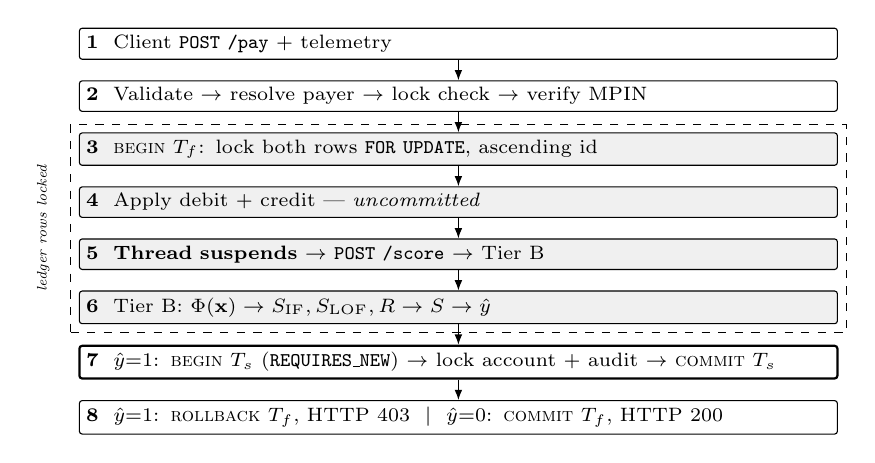
\begin{tikzpicture}[
  node distance=2.6mm,
  font=\scriptsize,
  box/.style={draw, rounded corners=1pt, align=left,
              text width=0.78\columnwidth, inner sep=2.4pt},
  crit/.style={box, fill=black!6},
  blk/.style={box, draw=black, thick},
  arrow/.style={-{Latex[length=1.3mm]}}
]
\node[box]  (n1) {\textbf{1}~~Client \texttt{POST /pay} $+$ telemetry};
\node[box, below=of n1] (n2) {\textbf{2}~~Validate $\rightarrow$ resolve payer $\rightarrow$ lock check $\rightarrow$ verify MPIN};
\node[crit, below=of n2] (n3) {\textbf{3}~~\textsc{begin} $T_{f}$: lock both rows \texttt{FOR UPDATE}, ascending id};
\node[crit, below=of n3] (n4) {\textbf{4}~~Apply debit $+$ credit --- \emph{uncommitted}};
\node[crit, below=of n4] (n5) {\textbf{5}~~\textbf{Thread suspends} $\rightarrow$ \texttt{POST /score} $\rightarrow$ Tier~B};
\node[crit, below=of n5] (n6) {\textbf{6}~~Tier~B: $\Phi(\mathbf{x}) \rightarrow S_{\mathrm{IF}}, S_{\mathrm{LOF}}, R \rightarrow S \rightarrow \hat{y}$};
\node[blk,  below=of n6] (n7) {\textbf{7}~~$\hat{y}{=}1$: \textsc{begin} $T_{s}$ (\texttt{REQUIRES\_NEW}) $\rightarrow$ lock account $+$ audit $\rightarrow$ \textsc{commit} $T_{s}$};
\node[box,  below=of n7] (n8) {\textbf{8}~~$\hat{y}{=}1$: \textsc{rollback} $T_{f}$, HTTP~403 ~\textbar~ $\hat{y}{=}0$: \textsc{commit} $T_{f}$, HTTP~200};
\foreach \a/\b in {n1/n2, n2/n3, n3/n4, n4/n5, n5/n6, n6/n7, n7/n8}
  \draw[arrow] (\a) -- (\b);
\begin{scope}[on background layer]
  \node[draw, dashed, fit=(n3)(n4)(n5)(n6), inner sep=3pt] (win) {};
\end{scope}
\node[rotate=90, anchor=south, font=\tiny\itshape]
  at ([xshift=-1.4mm]win.west) {ledger rows locked};
\end{tikzpicture}
\caption{Switch-to-scorer execution lifecycle. Steps 3--6 execute with
both balance rows held under \texttt{PESSIMISTIC\_WRITE}. Step~7
commits on an independent connection and therefore survives the
rollback in step~8, establishing invariant~\eqref{eq:invariant}.}
\label{fig:lifecycle}
\end{figure}

%%=====================================================================
\section{Empirical Evaluation and Performance Analysis}
\label{sec:evaluation}

We evaluate three properties: the detection efficacy of each tier and
of their fusion, the behaviour of the decision boundary across the
amount domain, and the latency the pipeline imposes on a held database
lock. All results are reproducible from the repository under seed~$42$.

\subsection{Experimental Setup and Workload Synthesis}
\label{subsec:setup}

\subsubsection{Corpus and partition}
The corpus contains $250{,}000$ UPI transaction records. An $80/20$
split under seed~$42$ yields $200{,}000$ training rows and $50{,}000$
held-out clean rows. The embedding of \eqref{eq:phi} maps each record
to $d=67$ dimensions, of which $64$ are one-hot indicators. The LOF
reference set is $|\mathcal{R}| = 40{,}000$ points drawn uniformly
without replacement from the training partition.

\subsubsection{Rejection of the supplied labels}
The corpus ships a \texttt{fraud\_flag} column which we do not use as
ground truth. Scoring the flag against our detectors yields
ROC-AUC~$\approx 0.48$, statistically indistinguishable from random
assignment. Reporting supervised metrics against an uninformative
label would measure the label, not the detector. The flag is withheld
from every fitting procedure in this work.

\subsubsection{Perturbation-based fraud injection}
We construct ground truth by sampling real clean rows from the
held-out partition and overwriting only the fields that define each
fraud archetype; all remaining fields retain their sampled values, so
synthetics are not separable by an artefact of generation.
Table~\ref{tab:archetypes} defines the four archetypes, $100$ instances
each, giving an evaluation set of $50{,}000$ clean and $400$ injected
transactions at a prevalence of $0.79\%$.

\begin{table}[t]
\centering
\caption{Injected fraud archetypes. Archetype~B is a negative control.}
\label{tab:archetypes}
\renewcommand{\arraystretch}{1.2}
\footnotesize
\begin{tabular}{@{}cp{0.68\columnwidth}@{}}
\toprule
\textbf{ID} & \textbf{Perturbation} \\
\midrule
A & Off-hour drain: amount $\sim\mathcal{U}(25{,}000,\,60{,}000)$, hour $\in\{1,2,3,4\}$, P2P, Web \\
B & Velocity spike \emph{(negative control)}: amount $\sim\mathcal{U}(2{,}000,\,6{,}000)$, hour $\in\{13,\dots,16\}$, P2P, Android, 4G \\
C & Category anomaly: amount $\sim\mathcal{U}(50{,}000,\,100{,}000)$, Grocery, P2M, hour $\in[10,20]$ \\
D & Context anomaly: amount $\sim\mathcal{U}(2{,}000,\,9{,}000)$, hour $\in\{0,\dots,4\}$, P2P, Web, WiFi \\
\bottomrule
\end{tabular}
\end{table}

Archetype~B is included deliberately as a detector of methodological
error. A velocity attack is defined by the arrival rate of
individually unremarkable transfers, which is information no
per-transaction feature vector carries. A system reporting appreciable
recall on~B would indicate leakage in the injection procedure rather
than detection capability. Its expected recall is zero.

\subsubsection{Threshold calibration}
The operating threshold was fixed by sweeping the fused score and
selecting the value whose false-positive rate on the $50{,}000$ clean
rows equals the target $\mathrm{FPR}=0.0086$. The sweep returns
$\tau = 0.802$, the value serialised in the deployed bundle. All
comparisons in Section~\ref{subsec:ablation} are conducted at this
matched FPR, so differences in recall are not artefacts of differing
alert budgets.

\subsection{Detection Efficacy and Tier Ablation}
\label{subsec:ablation}

Table~\ref{tab:ablation} reports the four configurations. We include
false discovery rate, $\mathrm{FDR} = 1 - \mathrm{Precision}$, because
it states the operational cost directly: the fraction of raised alerts
that are wrong.

\begin{table}[t]
\centering
\caption{Tier ablation on the injected evaluation set. Learned
configurations are thresholded to a matched $\mathrm{FPR}=0.0086$.}
\label{tab:ablation}
\renewcommand{\arraystretch}{1.25}
\footnotesize
\setlength{\tabcolsep}{4pt}
\begin{tabular}{@{}lccccc@{}}
\toprule
\textbf{Configuration} & \textbf{P} & \textbf{R} & \textbf{F1} & \textbf{FDR} & \textbf{AUC} \\
\midrule
(a) Tier-1 rules only$^{\dagger}$          & $0.738$ & $0.500$ & $0.596$ & $0.262$ & --- \\
(b) Isolation Forest only                  & $0.121$ & $0.147$ & $0.133$ & $0.879$ & $0.7231$ \\
(c) LOF only ($k=20$)                      & $0.409$ & $0.745$ & $0.528$ & $0.591$ & $0.8959$ \\
(d) Fusion, no escalation                  & $0.409$ & $0.745$ & $0.528$ & $0.591$ & $0.8812$ \\
\midrule
(e) \textbf{RT-IIPF deployed}$^{\ddagger}$ & $0.380$ & $0.745$ & $0.503$ & $0.620$ & --- \\
\bottomrule
\end{tabular}

\vspace{2pt}
{\footnotesize\raggedright
$^{\dagger}$Rules emit a deterministic binary decision; their FPR is
$0.0014$ and is not tunable to the matched budget.
$^{\ddagger}$Fusion \eqref{eq:fused} with hard-rule escalation
\eqref{eq:hard}; measured FPR $0.0097$.\par}
\end{table}

Three findings follow, two of which are negative.

\subsubsection{The density tier carries the detection}
Configuration~(c) raises recall from $0.147$ to $0.745$ over
configuration~(b) at identical FPR, a factor of $5.07$. The gap is
explained by the geometry of \eqref{eq:dim}: with $64$ of $67$
coordinates binary and exactly $10$ non-zero per record, the
axis-parallel random splits of the forest fall predominantly on
all-zero coordinates and isolate little. The neighbour-based statistic
of \eqref{eq:lof} operates on the full coordinate vector
simultaneously and is unaffected by this sparsity.

\subsubsection{The forest contributes no detection}
Configurations~(c) and~(d) are identical in precision, recall, and F1
to three decimal places, and the per-archetype recalls in
Table~\ref{tab:archetype_recall} coincide exactly. Adding the forest at
$\omega_{\mathrm{IF}}=0.20$ changes no verdict on this evaluation set
while reducing ROC-AUC from $0.8959$ to $0.8812$. We report this as a
negative result: on one-hot-dominated payment features, a
partition-based detector fused with a density-based one supplies no
incremental detection, and consumes the largest single share of
inference time (Section~\ref{subsec:latency}).

\subsubsection{Rule escalation costs precision without adding recall}
Configuration~(e), the deployed system, holds recall at $0.745$ while
precision falls from $0.409$ to $0.380$ and FDR rises from $0.591$ to
$0.620$. The hard-rule disjunction of \eqref{eq:decide} therefore
raises additional alerts on this evaluation set without catching
additional injected frauds. We retain it on grounds the injected set
cannot measure: the rules remain valid beyond the training support
where \eqref{eq:S_IF} and \eqref{eq:S_LOF} saturate, they emit a
reason code, and they survive unavailability of the learned tiers.
Section~\ref{subsec:edge} quantifies a regime in which this matters.

\begin{table}[t]
\centering
\caption{Per-archetype recall. Archetype~B is the negative control.}
\label{tab:archetype_recall}
\renewcommand{\arraystretch}{1.2}
\footnotesize
\begin{tabular}{@{}lccc@{}}
\toprule
\textbf{Archetype} & \textbf{IF} & \textbf{LOF} & \textbf{Hybrid} \\
\midrule
A~~off-hour drain          & $0.26$ & $1.00$ & $1.00$ \\
B~~velocity (neg.\ ctrl.)  & $0.00$ & $0.01$ & $0.01$ \\
C~~category anomaly        & $0.07$ & $1.00$ & $1.00$ \\
D~~context anomaly         & $0.26$ & $0.97$ & $0.97$ \\
\bottomrule
\end{tabular}
\end{table}

Archetype~B returns recall $0.01$, within sampling noise of the
expected zero, which supports the injection procedure. Excluding~B,
the detectable population is $300$ transactions, of which the deployed
system identifies $297$, or $99.0\%$ of the attainable ceiling. The
aggregate recall of $0.745$ is bounded above by $0.75$ by
construction, since one quarter of the injected set is architecturally
undetectable by a per-transaction model. We report the unadjusted
figure and state the bound rather than excluding the control from the
denominator.

\subsection{Decision Boundary Across the Amount Domain}
\label{subsec:edge}

To isolate the effect of amount, we scored a sweep in which all twelve
non-amount features are held fixed (P2M, Grocery, Web, 4G, hour~$18$,
weekday) and only the transfer amount varies.
Table~\ref{tab:sweep} reports the live service response at each point.

\begin{table}[t]
\centering
\caption{Amount sweep with all other features held constant. Rule
thresholds from \eqref{eq:th1}--\eqref{eq:th3} are marked.}
\label{tab:sweep}
\renewcommand{\arraystretch}{1.2}
\footnotesize
\setlength{\tabcolsep}{4pt}
\begin{tabular}{@{}rccccl@{}}
\toprule
\textbf{Amount} & $S_{\mathrm{IF}}$ & $S_{\mathrm{LOF}}$ & $R$ & $S$ & \textbf{Verdict} \\
\midrule
$50$            & $0.467$ & $0.340$ & $0.00$ & $0.365$ & ALLOW \\
$1{,}000$       & $0.461$ & $0.357$ & $0.00$ & $0.377$ & ALLOW \\
$5{,}000$       & $0.531$ & $0.814$ & $0.00$ & $0.757$ & ALLOW \\
$8{,}998^{a}$   & $0.593$ & $0.568$ & $0.00$ & $0.573$ & ALLOW \\
$11{,}136^{b}$  & $0.617$ & $0.519$ & $0.20$ & $0.538$ & ALLOW \\
$16{,}450^{c}$  & $0.617$ & $0.474$ & $0.55$ & $0.550$ & \textbf{BLOCK} \\
$20{,}000$      & $0.617$ & $0.537$ & $1.00$ & $1.000$ & \textbf{BLOCK} \\
$50{,}000$      & $0.617$ & $1.000$ & $1.00$ & $1.000$ & \textbf{BLOCK} \\
\bottomrule
\end{tabular}

\vspace{2pt}
{\footnotesize\raggedright
Amounts in INR. $^{a}\theta_{\mathrm{high}}$,
$^{b}\theta_{\mathrm{tick}}$, $^{c}\theta_{\mathrm{ext}}$.\par}
\end{table}

\subsubsection{The learned score is not monotone in amount}
$S_{\mathrm{LOF}}$ attains $0.814$ at \INR{5{,}000} and falls to
$0.519$ at \INR{11{,}136}, a larger transfer in the same context. This
is the expected behaviour of a density statistic rather than a defect:
\eqref{eq:lof} measures neighbourhood sparsity, and \INR{5{,}000}
occupies a thinner region of the Grocery/P2M population than
\INR{11{,}136} does. A policy requiring that risk not decrease with
amount therefore cannot be expressed by the learned tiers alone.
Column~$R$ is monotone by construction and supplies that guarantee.

\subsubsection{The decision disjunction is not redundant}
At \INR{16{,}450} the system blocks with $S = 0.550$, which is below
$\tau = 0.802$. The verdict is produced entirely by the hard-rule
branch of \eqref{eq:decide}, triggered by $r_{1}$ at
$\theta_{\mathrm{ext}}$. This is the empirical demonstration that the
two branches of \eqref{eq:decide} are independent: a configuration
thresholding on $S$ alone would admit this transaction.

\subsubsection{Selectivity}
The \INR{50} and \INR{50{,}000} endpoints share an identical channel
context---same merchant category, device, network, hour, and both
counterparties---and differ only in amount, yet receive opposite
verdicts ($S=0.365$ versus $S=1.000$). The boundary is therefore
driven by the transaction, not by the channel: a Web-origin Grocery
payment is not rejected categorically. The first transition occurs at
$\theta_{\mathrm{ext}}$, between \INR{11{,}136} and \INR{16{,}450}.

\subsection{Latency and Lock Contention}
\label{subsec:latency}

We separate two deployment contexts, since conflating them would
misattribute platform cost to the algorithm.

\subsubsection{Component cost, laboratory host}
Table~\ref{tab:components} decomposes inference over $n=300$ warm
iterations.

\begin{table}[t]
\centering
\caption{Per-component inference latency, laboratory host, $n=300$.}
\label{tab:components}
\renewcommand{\arraystretch}{1.2}
\footnotesize
\begin{tabular}{@{}lrrrr@{}}
\toprule
\textbf{Component} & \textbf{Mean (ms)} & \textbf{p50} & \textbf{p95} & \textbf{Share} \\
\midrule
Isolation Forest (Tier 2) & $9.549$ & $9.513$ & $9.758$ & $55.1\%$ \\
Preprocessor $\Phi$       & $3.799$ & $3.600$ & $4.052$ & $21.9\%$ \\
LOF (Tier 3)              & $3.178$ & $3.128$ & $3.515$ & $18.3\%$ \\
Frame construction        & $0.610$ & $0.589$ & $0.721$ & $3.5\%$ \\
Rule engine (Tier 1)      & $0.193$ & $0.183$ & $0.254$ & $1.1\%$ \\
\midrule
\textbf{Total}            & $\mathbf{17.330}$ & & & $100\%$ \\
\bottomrule
\end{tabular}
\end{table}

The forest consumes $55.1\%$ of inference while contributing no
detection (Section~\ref{subsec:ablation}). Removing it would reduce
inference to approximately $7.8$\,ms at unchanged recall. We report the
deployed configuration as measured and identify this as the primary
available optimisation.

\subsubsection{End-to-end latency and the lock window}
At concurrency~$1$, where no queuing occurs, the switch completes a
payment in mean $22.4$\,ms (p50~$22.3$, p95~$23.8$, p99~$25.3$). The
difference against Table~\ref{tab:components} attributes
$\approx 5.1$\,ms to switch-side work: MPIN verification, lock
acquisition, JPA flush, and HTTP serialisation in both directions.

The lock-hold window spans steps 3--8 of Fig.~\ref{fig:lifecycle} and
is therefore bounded by
\begin{equation}
17.3~\mathrm{ms} \;\lesssim\; W_{\mathrm{lock}} \;\lesssim\; 22.4~\mathrm{ms},
\label{eq:lockwindow}
\end{equation}
with a hard ceiling of $1500$\,ms enforced by the read timeout of
Section~\ref{subsec:failclosed}. Equation~\eqref{eq:lockwindow} is the
quantity the architecture trades for pre-commit interception.

\subsubsection{Lock contention}
Table~\ref{tab:contention} compares an uncontended workload, in which
each virtual client holds a distinct account pair, against a contended
workload in which all clients compete for an overlapping account set.

\begin{table}[t]
\centering
\caption{Throughput under lock contention. Ratio $>1$ indicates the
contended workload was not slower.}
\label{tab:contention}
\renewcommand{\arraystretch}{1.2}
\footnotesize
\begin{tabular}{@{}rcccc@{}}
\toprule
\textbf{Clients} & \textbf{Uncont.\ (TPS)} & \textbf{Cont.\ (TPS)} & \textbf{Ratio} & \textbf{p95 (ms)} \\
\midrule
$1$  & $44.5$ & $47.2$ & $1.061$ & $23.8$  \\
$10$ & $49.2$ & $50.4$ & $1.024$ & $63.2$  \\
$25$ & $49.5$ & $50.6$ & $1.022$ & $374.5$ \\
$50$ & $50.0$ & $50.8$ & $1.016$ & $864.2$ \\
\bottomrule
\end{tabular}
\end{table}

Every ratio equals or exceeds unity: forcing all clients onto the same
ledger rows produced no measurable throughput penalty. The system is
not lock-bound. The binding constraint is the single-worker scoring
node of Section~\ref{subsec:resources}, which plateaus near $50$\,TPS
and saturates before lock queuing becomes observable. The ordering
discipline of \eqref{eq:lockorder} held throughout; no deadlock
occurred across the full benchmark.

Measured p95 remains within the $500$\,ms budget of
Section~\ref{subsec:intro_constraints} up to $25$ concurrent clients
and exceeds it at $50$, which bounds the operating envelope of a
single-worker deployment. We note a tail effect visible at
concurrency~$\geq 10$: p99 reaches $3.9$--$4.0$\,s in \emph{both}
workloads while p95 remains below $65$\,ms at concurrency~$10$. Its
equal magnitude under both conditions indicates client-side connection
queuing against the saturated scorer rather than lock waiting.

\subsubsection{Cloud deployment}
On a $512$\,MB shared-CPU container, warm scorer-internal inference
measures mean $178.1$\,ms over $n=9$ samples (range
$101.4$--$235.1$\,ms), approximately $10\times$ the laboratory figure
in Table~\ref{tab:components}. The gap is attributable to CPU
provisioning, not to the algorithm or to HTTP transport. Observed
end-to-end switch latencies on the deployed instance were $337$\,ms and
$410$\,ms; a larger sample is required before reporting percentiles.

A single cold-start observation of $13{,}298$\,ms was recorded as the
first request after container idle eviction. This figure measures
platform container startup plus the $\approx 1.8$\,s bundle load, and
is excluded from steady-state analysis. It is reported because the
fail-closed policy of Section~\ref{subsec:failclosed} converts a cold
start into an HTTP~$503$ rejection, which is a deployment
consideration for platforms that evict idle containers.

%%=====================================================================
\section{Conclusion and Future Work}
\label{sec:conclusion}

We implemented and measured a fraud control that executes inside the
database transaction, while both ledger rows are held under write
locks and the debit is uncommitted. A fraudulent transfer is rolled
back atomically and never persists in the ledger, while the account
lock and audit record commit through an independent transaction and
survive that rollback---invariant~\eqref{eq:invariant}, verified
experimentally. The inline cost is $17.3$\,ms of inference within a
$22.4$\,ms end-to-end path at unit concurrency, and a lock window
bounded by \eqref{eq:lockwindow}.

\subsection{Summary of Empirical Findings}

The division of labour between tiers is not the one the design
anticipated, and we state it as measured.

\textbf{Detection is carried entirely by the density estimator.} LOF
alone attains recall $0.745$ against $0.147$ for the forest at matched
FPR, a factor of $5.07$, and the fused configuration reproduces LOF's
precision, recall, and F1 to three decimal places. The forest changes
no verdict on our evaluation set while consuming $55.1\%$ of inference
time and reducing ROC-AUC from $0.8959$ to $0.8812$. The explanation is
geometric: with $64$ of $67$ coordinates one-hot and $10$ non-zero per
record, axis-parallel random partitioning has little to cut.

\textbf{The rule tier buys bounds, not recall.} Escalation reduces
precision from $0.409$ to $0.380$ at unchanged recall, so on the
injected set it is a net cost. Its value lies in three properties that
set cannot measure. It remains valid beyond the training support where
both learned scores saturate at unity. It emits a reason code naming
the predicate and threshold that fired, which an operator can act on
and an auditor can reconstruct. And it enforces monotonicity in amount
that the learned tiers demonstrably lack: Table~\ref{tab:sweep} shows
$S_{\mathrm{LOF}}$ \emph{falling} from $0.814$ to $0.519$ as the
transfer grows from \INR{5{,}000} to \INR{11{,}136}. The
\INR{16{,}450} row, blocked at $S = 0.550 < \tau$ by the hard-rule
branch alone, is the operating point at which that guarantee binds.

\textbf{The system is not lock-bound.} Contended and uncontended
throughput are statistically indistinguishable across all
concurrencies tested (ratios $1.016$--$1.061$), with no deadlock under
the ordering discipline of \eqref{eq:lockorder}. The binding
constraint is the single-worker scoring node, which plateaus near
$50$\,TPS and keeps p95 within the $500$\,ms budget up to $25$
concurrent clients.

\subsection{Limitations}

The feature vector is strictly per-transaction, so velocity attacks are
architecturally undetectable; archetype~B quantifies this at recall
$0.01$ and bounds aggregate recall above by $0.75$ by construction.
Ground truth is synthetic, since the corpus labels are uninformative
(ROC-AUC~$\approx 0.48$); the injected archetypes encode our
assumptions about fraud rather than confirmed cases. The LOF
calibration anchors are computed on the same reference set the
estimator is fitted on. The embedded database preserves the audit
trail for the process lifetime only, and the switch implements no
request-deduplication key. Results derive from one corpus and one
geography.

\subsection{Future Work}

\subsubsection{Transport for the tail}
The p99 of $3.9$--$4.0$\,s at concurrency~$\geq 10$ is connection
queuing against a saturated single-worker scorer, not lock waiting.
Replacing synchronous HTTP/REST with multiplexed gRPC over Protocol
Buffers would remove per-request connection establishment and head-of-line
blocking, and eliminate JSON serialisation from a path where
Table~\ref{tab:components} already attributes measurable cost to frame
construction. The expected effect is on the tail rather than the
median, which is the operationally relevant quantity given that
\eqref{eq:ordering} holds locks for the full round trip.

\subsubsection{Distributed and non-stationary reference clusters}
The reference set $\mathcal{R}$ is sampled once and frozen, so the
density estimate ages as transaction behaviour drifts, and
$\mathcal{O}(|\mathcal{R}|d)$ per query bounds how large it may grow.
Two directions follow: approximate nearest-neighbour indexing to
decouple query cost from $|\mathcal{R}|$, and a sharded reference set
refreshed on a rolling window, which raises the question of
consistency between replicas holding different reference states while
\eqref{eq:decide} requires reproducible verdicts for audit.

\subsubsection{Identity-bearing features}
The client captures a device signature and a coarse location hash that
the switch validates but never forwards to the model; only device
\emph{type} and network type enter $\mathbf{x}$. Persisting signatures
per account would admit an \texttt{is\_new\_device} feature and address
the social-engineering case, in which the victim authorises the
payment from their own device and every present feature appears
normal.

\subsubsection{Graduated response}
The present policy is binary. Routing scores in a band below $\tau$ to
out-of-band re-authentication rather than to rejection would convert a
portion of the $0.620$ false discovery rate from blocked legitimate
payments into a challenge, at the cost of extending the lock window or
releasing it pending the challenge---a trade-off that interacts
directly with \eqref{eq:ordering}.

\subsubsection{Removing the forest}
Configurations~(c) and~(d) of Table~\ref{tab:ablation} are
indistinguishable in detection. Dropping Tier~2 would reduce inference
from $17.3$\,ms to approximately $7.8$\,ms at unchanged recall. We did
not adopt this for the reported system because the measurement
postdates deployment, and re-validation against the full benchmark
remains outstanding.

%%=====================================================================
\bibliographystyle{IEEEtran}
\bibliography{references}

\end{document}
